% Created by tikzDevice version 0.12 on 2020-02-28 11:03:25
% !TEX encoding = UTF-8 Unicode
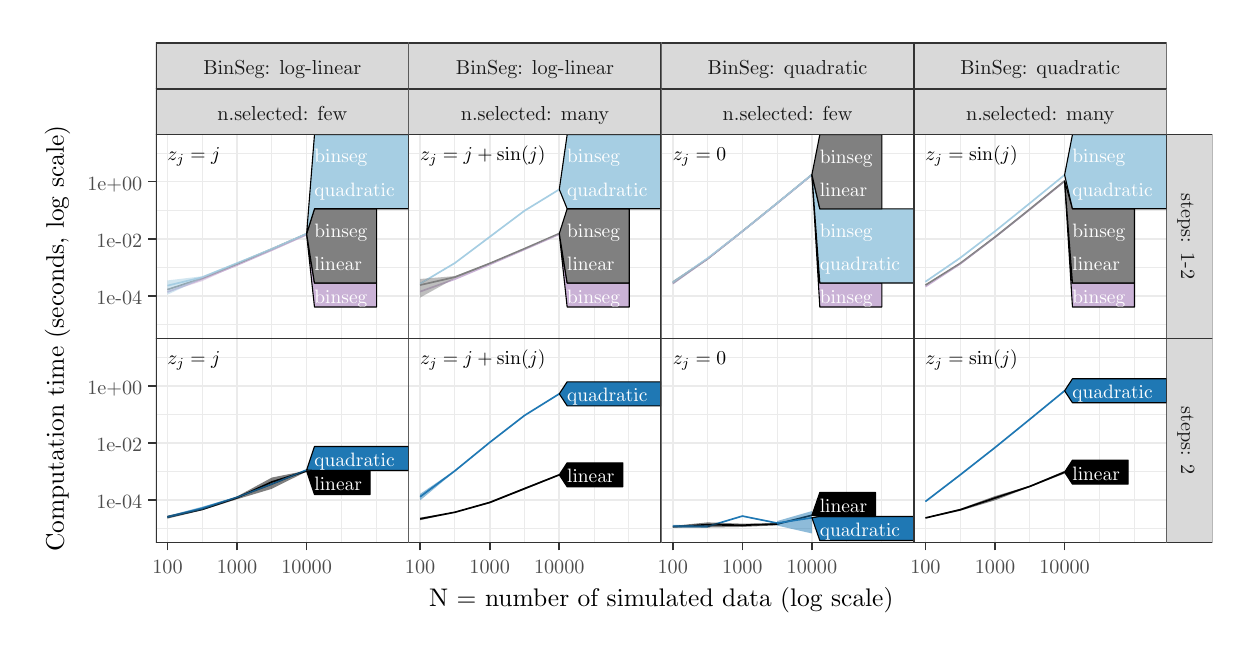
\begin{tikzpicture}[x=1pt,y=1pt]
\definecolor{fillColor}{RGB}{255,255,255}
\path[use as bounding box,fill=fillColor,fill opacity=0.00] (0,0) rectangle (433.62,216.81);
\begin{scope}
\path[clip] (  0.00,  0.00) rectangle (433.62,216.81);
\definecolor{drawColor}{RGB}{255,255,255}
\definecolor{fillColor}{RGB}{255,255,255}

\path[draw=drawColor,line width= 0.6pt,line join=round,line cap=round,fill=fillColor] (  0.00,  0.00) rectangle (433.62,216.81);
\end{scope}
\begin{scope}
\path[clip] ( 46.36,104.43) rectangle (137.66,178.17);
\definecolor{fillColor}{RGB}{255,255,255}

\path[fill=fillColor] ( 46.36,104.43) rectangle (137.66,178.17);
\definecolor{drawColor}{gray}{0.92}

\path[draw=drawColor,line width= 0.3pt,line join=round] ( 46.36,109.61) --
	(137.66,109.61);

\path[draw=drawColor,line width= 0.3pt,line join=round] ( 46.36,130.23) --
	(137.66,130.23);

\path[draw=drawColor,line width= 0.3pt,line join=round] ( 46.36,150.85) --
	(137.66,150.85);

\path[draw=drawColor,line width= 0.3pt,line join=round] ( 46.36,171.48) --
	(137.66,171.48);

\path[draw=drawColor,line width= 0.3pt,line join=round] ( 63.09,104.43) --
	( 63.09,178.17);

\path[draw=drawColor,line width= 0.3pt,line join=round] ( 88.23,104.43) --
	( 88.23,178.17);

\path[draw=drawColor,line width= 0.3pt,line join=round] (113.37,104.43) --
	(113.37,178.17);

\path[draw=drawColor,line width= 0.3pt,line join=round] (125.94,104.43) --
	(125.94,178.17);

\path[draw=drawColor,line width= 0.6pt,line join=round] ( 46.36,119.92) --
	(137.66,119.92);

\path[draw=drawColor,line width= 0.6pt,line join=round] ( 46.36,140.54) --
	(137.66,140.54);

\path[draw=drawColor,line width= 0.6pt,line join=round] ( 46.36,161.17) --
	(137.66,161.17);

\path[draw=drawColor,line width= 0.6pt,line join=round] ( 50.51,104.43) --
	( 50.51,178.17);

\path[draw=drawColor,line width= 0.6pt,line join=round] ( 75.66,104.43) --
	( 75.66,178.17);

\path[draw=drawColor,line width= 0.6pt,line join=round] (100.80,104.43) --
	(100.80,178.17);
\definecolor{drawColor}{RGB}{0,0,0}

\node[text=drawColor,anchor=base west,inner sep=0pt, outer sep=0pt, scale=  0.71] at ( 50.51,168.94) {$z_j = j$};
\definecolor{drawColor}{RGB}{202,178,214}

\path[draw=drawColor,line width= 0.6pt,line join=round] ( 50.51,121.29) --
	( 63.09,126.00) --
	( 75.66,131.03) --
	( 88.23,136.43) --
	(100.80,142.01);
\definecolor{drawColor}{gray}{0.50}

\path[draw=drawColor,line width= 0.6pt,line join=round] ( 50.51,122.17) --
	( 63.09,126.27) --
	( 75.66,131.47) --
	( 88.23,136.83) --
	(100.80,142.32);
\definecolor{drawColor}{RGB}{166,206,227}

\path[draw=drawColor,line width= 0.6pt,line join=round] ( 50.51,123.60) --
	( 63.09,126.61) --
	( 75.66,131.69) --
	( 88.23,136.85) --
	(100.80,142.35);
\definecolor{fillColor}{RGB}{202,178,214}

\path[fill=fillColor,fill opacity=0.50] ( 50.51,121.40) --
	( 63.09,126.66) --
	( 75.66,131.16) --
	( 88.23,136.46) --
	(100.80,142.17) --
	(100.80,141.85) --
	( 88.23,136.40) --
	( 75.66,130.90) --
	( 63.09,125.23) --
	( 50.51,121.18) --
	cycle;
\definecolor{fillColor}{RGB}{127,127,127}

\path[fill=fillColor,fill opacity=0.50] ( 50.51,122.29) --
	( 63.09,126.33) --
	( 75.66,131.66) --
	( 88.23,136.87) --
	(100.80,142.34) --
	(100.80,142.29) --
	( 88.23,136.79) --
	( 75.66,131.28) --
	( 63.09,126.20) --
	( 50.51,122.03) --
	cycle;
\definecolor{fillColor}{RGB}{166,206,227}

\path[fill=fillColor,fill opacity=0.50] ( 50.51,125.47) --
	( 63.09,126.98) --
	( 75.66,132.04) --
	( 88.23,136.88) --
	(100.80,142.40) --
	(100.80,142.30) --
	( 88.23,136.83) --
	( 75.66,131.31) --
	( 63.09,126.21) --
	( 50.51,120.31) --
	cycle;
\end{scope}
\begin{scope}
\path[clip] ( 46.36,104.43) rectangle (137.66,178.17);
\definecolor{drawColor}{RGB}{0,0,0}
\definecolor{fillColor}{RGB}{202,178,214}

\path[draw=drawColor,line width= 0.4pt,line join=round,line cap=round,fill=fillColor] (100.80,142.01) --
	(103.64,124.54) --
	(126.08,124.54) --
	(126.08,115.86) --
	(103.64,115.86) --
	cycle;
\definecolor{fillColor}{gray}{0.50}

\path[draw=drawColor,line width= 0.4pt,line join=round,line cap=round,fill=fillColor] (100.80,142.32) --
	(103.64,151.36) --
	(126.08,151.36) --
	(126.08,124.54) --
	(103.64,124.54) --
	cycle;
\definecolor{fillColor}{RGB}{166,206,227}

\path[draw=drawColor,line width= 0.4pt,line join=round,line cap=round,fill=fillColor] (100.80,142.35) --
	(103.64,178.17) --
	(137.66,178.17) --
	(137.66,151.36) --
	(103.64,151.36) --
	cycle;
\definecolor{drawColor}{RGB}{255,255,255}

\node[text=drawColor,anchor=base west,inner sep=0pt, outer sep=0pt, scale=  0.70] at (103.64,117.31) {binseg};

\node[text=drawColor,anchor=base west,inner sep=0pt, outer sep=0pt, scale=  0.70] at (103.64,141.10) {binseg};

\node[text=drawColor,anchor=base west,inner sep=0pt, outer sep=0pt, scale=  0.70] at (103.64,129.01) {linear};

\node[text=drawColor,anchor=base west,inner sep=0pt, outer sep=0pt, scale=  0.70] at (103.64,167.92) {binseg};

\node[text=drawColor,anchor=base west,inner sep=0pt, outer sep=0pt, scale=  0.70] at (103.64,155.83) {quadratic};
\definecolor{drawColor}{gray}{0.20}

\path[draw=drawColor,line width= 0.6pt,line join=round,line cap=round] ( 46.36,104.43) rectangle (137.66,178.17);
\end{scope}
\begin{scope}
\path[clip] ( 46.36, 30.69) rectangle (137.66,104.43);
\definecolor{fillColor}{RGB}{255,255,255}

\path[fill=fillColor] ( 46.36, 30.69) rectangle (137.66,104.43);
\definecolor{drawColor}{gray}{0.92}

\path[draw=drawColor,line width= 0.3pt,line join=round] ( 46.36, 35.87) --
	(137.66, 35.87);

\path[draw=drawColor,line width= 0.3pt,line join=round] ( 46.36, 56.49) --
	(137.66, 56.49);

\path[draw=drawColor,line width= 0.3pt,line join=round] ( 46.36, 77.11) --
	(137.66, 77.11);

\path[draw=drawColor,line width= 0.3pt,line join=round] ( 46.36, 97.74) --
	(137.66, 97.74);

\path[draw=drawColor,line width= 0.3pt,line join=round] ( 63.09, 30.69) --
	( 63.09,104.43);

\path[draw=drawColor,line width= 0.3pt,line join=round] ( 88.23, 30.69) --
	( 88.23,104.43);

\path[draw=drawColor,line width= 0.3pt,line join=round] (113.37, 30.69) --
	(113.37,104.43);

\path[draw=drawColor,line width= 0.3pt,line join=round] (125.94, 30.69) --
	(125.94,104.43);

\path[draw=drawColor,line width= 0.6pt,line join=round] ( 46.36, 46.18) --
	(137.66, 46.18);

\path[draw=drawColor,line width= 0.6pt,line join=round] ( 46.36, 66.80) --
	(137.66, 66.80);

\path[draw=drawColor,line width= 0.6pt,line join=round] ( 46.36, 87.43) --
	(137.66, 87.43);

\path[draw=drawColor,line width= 0.6pt,line join=round] ( 50.51, 30.69) --
	( 50.51,104.43);

\path[draw=drawColor,line width= 0.6pt,line join=round] ( 75.66, 30.69) --
	( 75.66,104.43);

\path[draw=drawColor,line width= 0.6pt,line join=round] (100.80, 30.69) --
	(100.80,104.43);
\definecolor{drawColor}{RGB}{0,0,0}

\node[text=drawColor,anchor=base west,inner sep=0pt, outer sep=0pt, scale=  0.71] at ( 50.51, 95.20) {$z_j = j$};

\path[draw=drawColor,line width= 0.6pt,line join=round] ( 50.51, 39.97) --
	( 63.09, 42.76) --
	( 75.66, 46.94) --
	( 88.23, 52.65) --
	(100.80, 56.60);
\definecolor{drawColor}{RGB}{31,120,180}

\path[draw=drawColor,line width= 0.6pt,line join=round] ( 50.51, 40.02) --
	( 63.09, 43.18) --
	( 75.66, 47.12) --
	( 88.23, 51.89) --
	(100.80, 56.99);
\definecolor{fillColor}{RGB}{0,0,0}

\path[fill=fillColor,fill opacity=0.50] ( 50.51, 40.47) --
	( 63.09, 43.06) --
	( 75.66, 47.41) --
	( 88.23, 54.24) --
	(100.80, 56.75) --
	(100.80, 56.45) --
	( 88.23, 50.18) --
	( 75.66, 46.41) --
	( 63.09, 42.43) --
	( 50.51, 39.40) --
	cycle;
\definecolor{fillColor}{RGB}{31,120,180}

\path[fill=fillColor,fill opacity=0.50] ( 50.51, 40.37) --
	( 63.09, 43.70) --
	( 75.66, 47.32) --
	( 88.23, 52.11) --
	(100.80, 57.06) --
	(100.80, 56.93) --
	( 88.23, 51.67) --
	( 75.66, 46.92) --
	( 63.09, 42.61) --
	( 50.51, 39.64) --
	cycle;
\end{scope}
\begin{scope}
\path[clip] ( 46.36, 30.69) rectangle (137.66,104.43);
\definecolor{drawColor}{RGB}{0,0,0}
\definecolor{fillColor}{RGB}{0,0,0}

\path[draw=drawColor,line width= 0.4pt,line join=round,line cap=round,fill=fillColor] (100.80, 56.60) --
	(103.64, 56.80) --
	(123.75, 56.80) --
	(123.75, 48.12) --
	(103.64, 48.12) --
	cycle;
\definecolor{fillColor}{RGB}{31,120,180}

\path[draw=drawColor,line width= 0.4pt,line join=round,line cap=round,fill=fillColor] (100.80, 56.99) --
	(103.64, 65.47) --
	(137.66, 65.47) --
	(137.66, 56.80) --
	(103.64, 56.80) --
	cycle;
\definecolor{drawColor}{RGB}{255,255,255}

\node[text=drawColor,anchor=base west,inner sep=0pt, outer sep=0pt, scale=  0.70] at (103.64, 49.56) {linear};

\node[text=drawColor,anchor=base west,inner sep=0pt, outer sep=0pt, scale=  0.70] at (103.64, 58.24) {quadratic};
\definecolor{drawColor}{gray}{0.20}

\path[draw=drawColor,line width= 0.6pt,line join=round,line cap=round] ( 46.36, 30.69) rectangle (137.66,104.43);
\end{scope}
\begin{scope}
\path[clip] (137.66,104.43) rectangle (228.96,178.17);
\definecolor{fillColor}{RGB}{255,255,255}

\path[fill=fillColor] (137.66,104.43) rectangle (228.96,178.17);
\definecolor{drawColor}{gray}{0.92}

\path[draw=drawColor,line width= 0.3pt,line join=round] (137.66,109.61) --
	(228.96,109.61);

\path[draw=drawColor,line width= 0.3pt,line join=round] (137.66,130.23) --
	(228.96,130.23);

\path[draw=drawColor,line width= 0.3pt,line join=round] (137.66,150.85) --
	(228.96,150.85);

\path[draw=drawColor,line width= 0.3pt,line join=round] (137.66,171.48) --
	(228.96,171.48);

\path[draw=drawColor,line width= 0.3pt,line join=round] (154.38,104.43) --
	(154.38,178.17);

\path[draw=drawColor,line width= 0.3pt,line join=round] (179.52,104.43) --
	(179.52,178.17);

\path[draw=drawColor,line width= 0.3pt,line join=round] (204.67,104.43) --
	(204.67,178.17);

\path[draw=drawColor,line width= 0.3pt,line join=round] (217.24,104.43) --
	(217.24,178.17);

\path[draw=drawColor,line width= 0.6pt,line join=round] (137.66,119.92) --
	(228.96,119.92);

\path[draw=drawColor,line width= 0.6pt,line join=round] (137.66,140.54) --
	(228.96,140.54);

\path[draw=drawColor,line width= 0.6pt,line join=round] (137.66,161.17) --
	(228.96,161.17);

\path[draw=drawColor,line width= 0.6pt,line join=round] (141.81,104.43) --
	(141.81,178.17);

\path[draw=drawColor,line width= 0.6pt,line join=round] (166.95,104.43) --
	(166.95,178.17);

\path[draw=drawColor,line width= 0.6pt,line join=round] (192.10,104.43) --
	(192.10,178.17);
\definecolor{drawColor}{RGB}{0,0,0}

\node[text=drawColor,anchor=base west,inner sep=0pt, outer sep=0pt, scale=  0.71] at (141.81,168.94) {$z_j = j+\sin(j)$};
\definecolor{drawColor}{RGB}{202,178,214}

\path[draw=drawColor,line width= 0.6pt,line join=round] (141.81,121.44) --
	(154.38,125.94) --
	(166.95,131.23) --
	(179.52,136.67) --
	(192.10,142.17);
\definecolor{drawColor}{gray}{0.50}

\path[draw=drawColor,line width= 0.6pt,line join=round] (141.81,123.80) --
	(154.38,126.68) --
	(166.95,131.62) --
	(179.52,136.95) --
	(192.10,142.43);
\definecolor{drawColor}{RGB}{166,206,227}

\path[draw=drawColor,line width= 0.6pt,line join=round] (141.81,124.30) --
	(154.38,131.77) --
	(166.95,141.21) --
	(179.52,150.65) --
	(192.10,158.36);
\definecolor{fillColor}{RGB}{202,178,214}

\path[fill=fillColor,fill opacity=0.50] (141.81,121.48) --
	(154.38,126.01) --
	(166.95,131.31) --
	(179.52,136.69) --
	(192.10,142.31) --
	(192.10,142.03) --
	(179.52,136.66) --
	(166.95,131.15) --
	(154.38,125.88) --
	(141.81,121.41) --
	cycle;
\definecolor{fillColor}{RGB}{127,127,127}

\path[fill=fillColor,fill opacity=0.50] (141.81,126.00) --
	(154.38,127.05) --
	(166.95,131.77) --
	(179.52,136.98) --
	(192.10,142.52) --
	(192.10,142.35) --
	(179.52,136.92) --
	(166.95,131.46) --
	(154.38,126.27) --
	(141.81,119.27) --
	cycle;
\definecolor{fillColor}{RGB}{166,206,227}

\path[fill=fillColor,fill opacity=0.50] (141.81,124.42) --
	(154.38,131.85) --
	(166.95,141.28) --
	(179.52,150.73) --
	(192.10,158.37) --
	(192.10,158.36) --
	(179.52,150.57) --
	(166.95,141.13) --
	(154.38,131.70) --
	(141.81,124.19) --
	cycle;
\end{scope}
\begin{scope}
\path[clip] (137.66,104.43) rectangle (228.96,178.17);
\definecolor{drawColor}{RGB}{0,0,0}
\definecolor{fillColor}{RGB}{202,178,214}

\path[draw=drawColor,line width= 0.4pt,line join=round,line cap=round,fill=fillColor] (192.10,142.17) --
	(194.94,124.54) --
	(217.37,124.54) --
	(217.37,115.86) --
	(194.94,115.86) --
	cycle;
\definecolor{fillColor}{gray}{0.50}

\path[draw=drawColor,line width= 0.4pt,line join=round,line cap=round,fill=fillColor] (192.10,142.43) --
	(194.94,151.36) --
	(217.37,151.36) --
	(217.37,124.54) --
	(194.94,124.54) --
	cycle;
\definecolor{fillColor}{RGB}{166,206,227}

\path[draw=drawColor,line width= 0.4pt,line join=round,line cap=round,fill=fillColor] (192.10,158.36) --
	(194.94,178.17) --
	(228.96,178.17) --
	(228.96,151.36) --
	(194.94,151.36) --
	cycle;
\definecolor{drawColor}{RGB}{255,255,255}

\node[text=drawColor,anchor=base west,inner sep=0pt, outer sep=0pt, scale=  0.70] at (194.94,117.31) {binseg};

\node[text=drawColor,anchor=base west,inner sep=0pt, outer sep=0pt, scale=  0.70] at (194.94,141.10) {binseg};

\node[text=drawColor,anchor=base west,inner sep=0pt, outer sep=0pt, scale=  0.70] at (194.94,129.01) {linear};

\node[text=drawColor,anchor=base west,inner sep=0pt, outer sep=0pt, scale=  0.70] at (194.94,167.92) {binseg};

\node[text=drawColor,anchor=base west,inner sep=0pt, outer sep=0pt, scale=  0.70] at (194.94,155.83) {quadratic};
\definecolor{drawColor}{gray}{0.20}

\path[draw=drawColor,line width= 0.6pt,line join=round,line cap=round] (137.66,104.43) rectangle (228.96,178.17);
\end{scope}
\begin{scope}
\path[clip] (137.66, 30.69) rectangle (228.96,104.43);
\definecolor{fillColor}{RGB}{255,255,255}

\path[fill=fillColor] (137.66, 30.69) rectangle (228.96,104.43);
\definecolor{drawColor}{gray}{0.92}

\path[draw=drawColor,line width= 0.3pt,line join=round] (137.66, 35.87) --
	(228.96, 35.87);

\path[draw=drawColor,line width= 0.3pt,line join=round] (137.66, 56.49) --
	(228.96, 56.49);

\path[draw=drawColor,line width= 0.3pt,line join=round] (137.66, 77.11) --
	(228.96, 77.11);

\path[draw=drawColor,line width= 0.3pt,line join=round] (137.66, 97.74) --
	(228.96, 97.74);

\path[draw=drawColor,line width= 0.3pt,line join=round] (154.38, 30.69) --
	(154.38,104.43);

\path[draw=drawColor,line width= 0.3pt,line join=round] (179.52, 30.69) --
	(179.52,104.43);

\path[draw=drawColor,line width= 0.3pt,line join=round] (204.67, 30.69) --
	(204.67,104.43);

\path[draw=drawColor,line width= 0.3pt,line join=round] (217.24, 30.69) --
	(217.24,104.43);

\path[draw=drawColor,line width= 0.6pt,line join=round] (137.66, 46.18) --
	(228.96, 46.18);

\path[draw=drawColor,line width= 0.6pt,line join=round] (137.66, 66.80) --
	(228.96, 66.80);

\path[draw=drawColor,line width= 0.6pt,line join=round] (137.66, 87.43) --
	(228.96, 87.43);

\path[draw=drawColor,line width= 0.6pt,line join=round] (141.81, 30.69) --
	(141.81,104.43);

\path[draw=drawColor,line width= 0.6pt,line join=round] (166.95, 30.69) --
	(166.95,104.43);

\path[draw=drawColor,line width= 0.6pt,line join=round] (192.10, 30.69) --
	(192.10,104.43);
\definecolor{drawColor}{RGB}{0,0,0}

\node[text=drawColor,anchor=base west,inner sep=0pt, outer sep=0pt, scale=  0.71] at (141.81, 95.20) {$z_j = j+\sin(j)$};

\path[draw=drawColor,line width= 0.6pt,line join=round] (141.81, 39.32) --
	(154.38, 41.71) --
	(166.95, 45.24) --
	(179.52, 50.24) --
	(192.10, 55.23);
\definecolor{drawColor}{RGB}{31,120,180}

\path[draw=drawColor,line width= 0.6pt,line join=round] (141.81, 47.31) --
	(154.38, 56.67) --
	(166.95, 66.93) --
	(179.52, 76.67) --
	(192.10, 84.50);
\definecolor{fillColor}{RGB}{0,0,0}

\path[fill=fillColor,fill opacity=0.50] (141.81, 39.77) --
	(154.38, 41.81) --
	(166.95, 45.51) --
	(179.52, 50.56) --
	(192.10, 55.39) --
	(192.10, 55.07) --
	(179.52, 49.90) --
	(166.95, 44.95) --
	(154.38, 41.60) --
	(141.81, 38.83) --
	cycle;
\definecolor{fillColor}{RGB}{31,120,180}

\path[fill=fillColor,fill opacity=0.50] (141.81, 48.33) --
	(154.38, 56.87) --
	(166.95, 67.01) --
	(179.52, 76.76) --
	(192.10, 84.52) --
	(192.10, 84.48) --
	(179.52, 76.58) --
	(166.95, 66.86) --
	(154.38, 56.47) --
	(141.81, 45.99) --
	cycle;
\end{scope}
\begin{scope}
\path[clip] (137.66, 30.69) rectangle (228.96,104.43);
\definecolor{drawColor}{RGB}{0,0,0}
\definecolor{fillColor}{RGB}{0,0,0}

\path[draw=drawColor,line width= 0.4pt,line join=round,line cap=round,fill=fillColor] (192.10, 55.23) --
	(194.94, 59.57) --
	(215.04, 59.57) --
	(215.04, 50.89) --
	(194.94, 50.89) --
	cycle;
\definecolor{fillColor}{RGB}{31,120,180}

\path[draw=drawColor,line width= 0.4pt,line join=round,line cap=round,fill=fillColor] (192.10, 84.50) --
	(194.94, 88.84) --
	(228.96, 88.84) --
	(228.96, 80.16) --
	(194.94, 80.16) --
	cycle;
\definecolor{drawColor}{RGB}{255,255,255}

\node[text=drawColor,anchor=base west,inner sep=0pt, outer sep=0pt, scale=  0.70] at (194.94, 52.34) {linear};

\node[text=drawColor,anchor=base west,inner sep=0pt, outer sep=0pt, scale=  0.70] at (194.94, 81.61) {quadratic};
\definecolor{drawColor}{gray}{0.20}

\path[draw=drawColor,line width= 0.6pt,line join=round,line cap=round] (137.66, 30.69) rectangle (228.96,104.43);
\end{scope}
\begin{scope}
\path[clip] (228.96,104.43) rectangle (320.25,178.17);
\definecolor{fillColor}{RGB}{255,255,255}

\path[fill=fillColor] (228.96,104.43) rectangle (320.25,178.17);
\definecolor{drawColor}{gray}{0.92}

\path[draw=drawColor,line width= 0.3pt,line join=round] (228.96,109.61) --
	(320.25,109.61);

\path[draw=drawColor,line width= 0.3pt,line join=round] (228.96,130.23) --
	(320.25,130.23);

\path[draw=drawColor,line width= 0.3pt,line join=round] (228.96,150.85) --
	(320.25,150.85);

\path[draw=drawColor,line width= 0.3pt,line join=round] (228.96,171.48) --
	(320.25,171.48);

\path[draw=drawColor,line width= 0.3pt,line join=round] (245.68,104.43) --
	(245.68,178.17);

\path[draw=drawColor,line width= 0.3pt,line join=round] (270.82,104.43) --
	(270.82,178.17);

\path[draw=drawColor,line width= 0.3pt,line join=round] (295.96,104.43) --
	(295.96,178.17);

\path[draw=drawColor,line width= 0.3pt,line join=round] (308.53,104.43) --
	(308.53,178.17);

\path[draw=drawColor,line width= 0.6pt,line join=round] (228.96,119.92) --
	(320.25,119.92);

\path[draw=drawColor,line width= 0.6pt,line join=round] (228.96,140.54) --
	(320.25,140.54);

\path[draw=drawColor,line width= 0.6pt,line join=round] (228.96,161.17) --
	(320.25,161.17);

\path[draw=drawColor,line width= 0.6pt,line join=round] (233.11,104.43) --
	(233.11,178.17);

\path[draw=drawColor,line width= 0.6pt,line join=round] (258.25,104.43) --
	(258.25,178.17);

\path[draw=drawColor,line width= 0.6pt,line join=round] (283.39,104.43) --
	(283.39,178.17);
\definecolor{drawColor}{RGB}{0,0,0}

\node[text=drawColor,anchor=base west,inner sep=0pt, outer sep=0pt, scale=  0.71] at (233.11,168.94) {$z_j = 0$};
\definecolor{drawColor}{RGB}{202,178,214}

\path[draw=drawColor,line width= 0.6pt,line join=round] (233.11,124.35) --
	(245.68,133.25) --
	(258.25,143.16) --
	(270.82,153.30) --
	(283.39,163.60);
\definecolor{drawColor}{gray}{0.50}

\path[draw=drawColor,line width= 0.6pt,line join=round] (233.11,124.72) --
	(245.68,133.30) --
	(258.25,143.25) --
	(270.82,153.42) --
	(283.39,163.71);
\definecolor{drawColor}{RGB}{166,206,227}

\path[draw=drawColor,line width= 0.6pt,line join=round] (233.11,124.78) --
	(245.68,133.47) --
	(258.25,143.23) --
	(270.82,153.42) --
	(283.39,163.71);
\definecolor{fillColor}{RGB}{202,178,214}

\path[fill=fillColor,fill opacity=0.50] (233.11,124.70) --
	(245.68,133.42) --
	(258.25,143.25) --
	(270.82,153.31) --
	(283.39,163.65) --
	(283.39,163.55) --
	(270.82,153.28) --
	(258.25,143.06) --
	(245.68,133.07) --
	(233.11,123.96) --
	cycle;
\definecolor{fillColor}{RGB}{127,127,127}

\path[fill=fillColor,fill opacity=0.50] (233.11,125.28) --
	(245.68,133.34) --
	(258.25,143.28) --
	(270.82,153.43) --
	(283.39,163.72) --
	(283.39,163.70) --
	(270.82,153.41) --
	(258.25,143.21) --
	(245.68,133.25) --
	(233.11,124.09) --
	cycle;
\definecolor{fillColor}{RGB}{166,206,227}

\path[fill=fillColor,fill opacity=0.50] (233.11,125.21) --
	(245.68,133.66) --
	(258.25,143.25) --
	(270.82,153.43) --
	(283.39,163.71) --
	(283.39,163.70) --
	(270.82,153.41) --
	(258.25,143.21) --
	(245.68,133.28) --
	(233.11,124.31) --
	cycle;
\end{scope}
\begin{scope}
\path[clip] (228.96,104.43) rectangle (320.25,178.17);
\definecolor{drawColor}{RGB}{0,0,0}
\definecolor{fillColor}{RGB}{202,178,214}

\path[draw=drawColor,line width= 0.4pt,line join=round,line cap=round,fill=fillColor] (283.39,163.60) --
	(286.24,124.54) --
	(308.67,124.54) --
	(308.67,115.86) --
	(286.24,115.86) --
	cycle;
\definecolor{fillColor}{RGB}{166,206,227}

\path[draw=drawColor,line width= 0.4pt,line join=round,line cap=round,fill=fillColor] (283.39,163.71) --
	(286.24,151.35) --
	(320.25,151.35) --
	(320.25,124.54) --
	(286.24,124.54) --
	cycle;
\definecolor{fillColor}{gray}{0.50}

\path[draw=drawColor,line width= 0.4pt,line join=round,line cap=round,fill=fillColor] (283.39,163.71) --
	(286.24,178.17) --
	(308.67,178.17) --
	(308.67,151.35) --
	(286.24,151.35) --
	cycle;
\definecolor{drawColor}{RGB}{255,255,255}

\node[text=drawColor,anchor=base west,inner sep=0pt, outer sep=0pt, scale=  0.70] at (286.24,117.31) {binseg};

\node[text=drawColor,anchor=base west,inner sep=0pt, outer sep=0pt, scale=  0.70] at (286.24,141.10) {binseg};

\node[text=drawColor,anchor=base west,inner sep=0pt, outer sep=0pt, scale=  0.70] at (286.24,129.01) {quadratic};

\node[text=drawColor,anchor=base west,inner sep=0pt, outer sep=0pt, scale=  0.70] at (286.24,167.91) {binseg};

\node[text=drawColor,anchor=base west,inner sep=0pt, outer sep=0pt, scale=  0.70] at (286.24,155.82) {linear};
\definecolor{drawColor}{gray}{0.20}

\path[draw=drawColor,line width= 0.6pt,line join=round,line cap=round] (228.96,104.43) rectangle (320.25,178.17);
\end{scope}
\begin{scope}
\path[clip] (228.96, 30.69) rectangle (320.25,104.43);
\definecolor{fillColor}{RGB}{255,255,255}

\path[fill=fillColor] (228.96, 30.69) rectangle (320.25,104.43);
\definecolor{drawColor}{gray}{0.92}

\path[draw=drawColor,line width= 0.3pt,line join=round] (228.96, 35.87) --
	(320.25, 35.87);

\path[draw=drawColor,line width= 0.3pt,line join=round] (228.96, 56.49) --
	(320.25, 56.49);

\path[draw=drawColor,line width= 0.3pt,line join=round] (228.96, 77.11) --
	(320.25, 77.11);

\path[draw=drawColor,line width= 0.3pt,line join=round] (228.96, 97.74) --
	(320.25, 97.74);

\path[draw=drawColor,line width= 0.3pt,line join=round] (245.68, 30.69) --
	(245.68,104.43);

\path[draw=drawColor,line width= 0.3pt,line join=round] (270.82, 30.69) --
	(270.82,104.43);

\path[draw=drawColor,line width= 0.3pt,line join=round] (295.96, 30.69) --
	(295.96,104.43);

\path[draw=drawColor,line width= 0.3pt,line join=round] (308.53, 30.69) --
	(308.53,104.43);

\path[draw=drawColor,line width= 0.6pt,line join=round] (228.96, 46.18) --
	(320.25, 46.18);

\path[draw=drawColor,line width= 0.6pt,line join=round] (228.96, 66.80) --
	(320.25, 66.80);

\path[draw=drawColor,line width= 0.6pt,line join=round] (228.96, 87.43) --
	(320.25, 87.43);

\path[draw=drawColor,line width= 0.6pt,line join=round] (233.11, 30.69) --
	(233.11,104.43);

\path[draw=drawColor,line width= 0.6pt,line join=round] (258.25, 30.69) --
	(258.25,104.43);

\path[draw=drawColor,line width= 0.6pt,line join=round] (283.39, 30.69) --
	(283.39,104.43);
\definecolor{drawColor}{RGB}{0,0,0}

\node[text=drawColor,anchor=base west,inner sep=0pt, outer sep=0pt, scale=  0.71] at (233.11, 95.20) {$z_j = 0$};

\path[draw=drawColor,line width= 0.6pt,line join=round] (233.11, 36.49) --
	(245.68, 37.20) --
	(258.25, 37.03) --
	(270.82, 37.42) --
	(283.39, 40.62);
\definecolor{drawColor}{RGB}{31,120,180}

\path[draw=drawColor,line width= 0.6pt,line join=round] (233.11, 36.70) --
	(245.68, 36.56) --
	(258.25, 40.33) --
	(270.82, 37.79) --
	(283.39, 39.71);
\definecolor{fillColor}{RGB}{0,0,0}

\path[fill=fillColor,fill opacity=0.50] (233.11, 36.78) --
	(245.68, 38.04) --
	(258.25, 37.59) --
	(270.82, 37.81) --
	(270.82, 36.99) --
	(258.25, 36.40) --
	(245.68, 36.18) --
	(233.11, 36.18) --
	cycle;
\definecolor{fillColor}{RGB}{31,120,180}

\path[fill=fillColor,fill opacity=0.50] (233.11, 37.15) --
	(245.68, 36.92) --
	(245.68, 36.16) --
	(233.11, 36.20) --
	cycle;

\path[fill=fillColor,fill opacity=0.50] (270.82, 38.53) --
	(283.39, 42.14) --
	(283.39, 34.04) --
	(270.82, 36.90) --
	cycle;
\end{scope}
\begin{scope}
\path[clip] (228.96, 30.69) rectangle (320.25,104.43);
\definecolor{drawColor}{RGB}{0,0,0}
\definecolor{fillColor}{RGB}{31,120,180}

\path[draw=drawColor,line width= 0.4pt,line join=round,line cap=round,fill=fillColor] (283.39, 39.71) --
	(286.24, 40.17) --
	(320.25, 40.17) --
	(320.25, 31.49) --
	(286.24, 31.49) --
	cycle;
\definecolor{fillColor}{RGB}{0,0,0}

\path[draw=drawColor,line width= 0.4pt,line join=round,line cap=round,fill=fillColor] (283.39, 40.62) --
	(286.24, 48.85) --
	(306.34, 48.85) --
	(306.34, 40.17) --
	(286.24, 40.17) --
	cycle;
\definecolor{drawColor}{RGB}{255,255,255}

\node[text=drawColor,anchor=base west,inner sep=0pt, outer sep=0pt, scale=  0.70] at (286.24, 32.94) {quadratic};

\node[text=drawColor,anchor=base west,inner sep=0pt, outer sep=0pt, scale=  0.70] at (286.24, 41.61) {linear};
\definecolor{drawColor}{gray}{0.20}

\path[draw=drawColor,line width= 0.6pt,line join=round,line cap=round] (228.96, 30.69) rectangle (320.25,104.43);
\end{scope}
\begin{scope}
\path[clip] (320.25,104.43) rectangle (411.55,178.17);
\definecolor{fillColor}{RGB}{255,255,255}

\path[fill=fillColor] (320.25,104.43) rectangle (411.55,178.17);
\definecolor{drawColor}{gray}{0.92}

\path[draw=drawColor,line width= 0.3pt,line join=round] (320.25,109.61) --
	(411.55,109.61);

\path[draw=drawColor,line width= 0.3pt,line join=round] (320.25,130.23) --
	(411.55,130.23);

\path[draw=drawColor,line width= 0.3pt,line join=round] (320.25,150.85) --
	(411.55,150.85);

\path[draw=drawColor,line width= 0.3pt,line join=round] (320.25,171.48) --
	(411.55,171.48);

\path[draw=drawColor,line width= 0.3pt,line join=round] (336.97,104.43) --
	(336.97,178.17);

\path[draw=drawColor,line width= 0.3pt,line join=round] (362.12,104.43) --
	(362.12,178.17);

\path[draw=drawColor,line width= 0.3pt,line join=round] (387.26,104.43) --
	(387.26,178.17);

\path[draw=drawColor,line width= 0.3pt,line join=round] (399.83,104.43) --
	(399.83,178.17);

\path[draw=drawColor,line width= 0.6pt,line join=round] (320.25,119.92) --
	(411.55,119.92);

\path[draw=drawColor,line width= 0.6pt,line join=round] (320.25,140.54) --
	(411.55,140.54);

\path[draw=drawColor,line width= 0.6pt,line join=round] (320.25,161.17) --
	(411.55,161.17);

\path[draw=drawColor,line width= 0.6pt,line join=round] (324.40,104.43) --
	(324.40,178.17);

\path[draw=drawColor,line width= 0.6pt,line join=round] (349.55,104.43) --
	(349.55,178.17);

\path[draw=drawColor,line width= 0.6pt,line join=round] (374.69,104.43) --
	(374.69,178.17);
\definecolor{drawColor}{RGB}{0,0,0}

\node[text=drawColor,anchor=base west,inner sep=0pt, outer sep=0pt, scale=  0.71] at (324.40,168.94) {$z_j = \sin(j)$};
\definecolor{drawColor}{RGB}{202,178,214}

\path[draw=drawColor,line width= 0.6pt,line join=round] (324.40,123.23) --
	(336.97,131.47) --
	(349.55,141.06) --
	(362.12,151.12) --
	(374.69,161.32);
\definecolor{drawColor}{gray}{0.50}

\path[draw=drawColor,line width= 0.6pt,line join=round] (324.40,123.78) --
	(336.97,131.64) --
	(349.55,141.16) --
	(362.12,151.22) --
	(374.69,161.44);
\definecolor{drawColor}{RGB}{166,206,227}

\path[draw=drawColor,line width= 0.6pt,line join=round] (324.40,125.01) --
	(336.97,133.62) --
	(349.55,143.24) --
	(362.12,153.37) --
	(374.69,163.62);
\definecolor{fillColor}{RGB}{202,178,214}

\path[fill=fillColor,fill opacity=0.50] (324.40,123.29) --
	(336.97,131.57) --
	(349.55,141.08) --
	(362.12,151.13) --
	(374.69,161.33) --
	(374.69,161.31) --
	(362.12,151.11) --
	(349.55,141.04) --
	(336.97,131.36) --
	(324.40,123.17) --
	cycle;
\definecolor{fillColor}{RGB}{127,127,127}

\path[fill=fillColor,fill opacity=0.50] (324.40,123.84) --
	(336.97,131.69) --
	(349.55,141.20) --
	(362.12,151.24) --
	(374.69,161.44) --
	(374.69,161.43) --
	(362.12,151.21) --
	(349.55,141.13) --
	(336.97,131.58) --
	(324.40,123.73) --
	cycle;
\definecolor{fillColor}{RGB}{166,206,227}

\path[fill=fillColor,fill opacity=0.50] (324.40,125.22) --
	(336.97,133.88) --
	(349.55,143.25) --
	(362.12,153.39) --
	(374.69,163.64) --
	(374.69,163.60) --
	(362.12,153.35) --
	(349.55,143.22) --
	(336.97,133.35) --
	(324.40,124.79) --
	cycle;
\end{scope}
\begin{scope}
\path[clip] (320.25,104.43) rectangle (411.55,178.17);
\definecolor{drawColor}{RGB}{0,0,0}
\definecolor{fillColor}{RGB}{202,178,214}

\path[draw=drawColor,line width= 0.4pt,line join=round,line cap=round,fill=fillColor] (374.69,161.32) --
	(377.53,124.54) --
	(399.96,124.54) --
	(399.96,115.86) --
	(377.53,115.86) --
	cycle;
\definecolor{fillColor}{gray}{0.50}

\path[draw=drawColor,line width= 0.4pt,line join=round,line cap=round,fill=fillColor] (374.69,161.44) --
	(377.53,151.36) --
	(399.96,151.36) --
	(399.96,124.54) --
	(377.53,124.54) --
	cycle;
\definecolor{fillColor}{RGB}{166,206,227}

\path[draw=drawColor,line width= 0.4pt,line join=round,line cap=round,fill=fillColor] (374.69,163.62) --
	(377.53,178.17) --
	(411.55,178.17) --
	(411.55,151.36) --
	(377.53,151.36) --
	cycle;
\definecolor{drawColor}{RGB}{255,255,255}

\node[text=drawColor,anchor=base west,inner sep=0pt, outer sep=0pt, scale=  0.70] at (377.53,117.31) {binseg};

\node[text=drawColor,anchor=base west,inner sep=0pt, outer sep=0pt, scale=  0.70] at (377.53,141.10) {binseg};

\node[text=drawColor,anchor=base west,inner sep=0pt, outer sep=0pt, scale=  0.70] at (377.53,129.01) {linear};

\node[text=drawColor,anchor=base west,inner sep=0pt, outer sep=0pt, scale=  0.70] at (377.53,167.92) {binseg};

\node[text=drawColor,anchor=base west,inner sep=0pt, outer sep=0pt, scale=  0.70] at (377.53,155.83) {quadratic};
\definecolor{drawColor}{gray}{0.20}

\path[draw=drawColor,line width= 0.6pt,line join=round,line cap=round] (320.25,104.43) rectangle (411.55,178.17);
\end{scope}
\begin{scope}
\path[clip] (320.25, 30.69) rectangle (411.55,104.43);
\definecolor{fillColor}{RGB}{255,255,255}

\path[fill=fillColor] (320.25, 30.69) rectangle (411.55,104.43);
\definecolor{drawColor}{gray}{0.92}

\path[draw=drawColor,line width= 0.3pt,line join=round] (320.25, 35.87) --
	(411.55, 35.87);

\path[draw=drawColor,line width= 0.3pt,line join=round] (320.25, 56.49) --
	(411.55, 56.49);

\path[draw=drawColor,line width= 0.3pt,line join=round] (320.25, 77.11) --
	(411.55, 77.11);

\path[draw=drawColor,line width= 0.3pt,line join=round] (320.25, 97.74) --
	(411.55, 97.74);

\path[draw=drawColor,line width= 0.3pt,line join=round] (336.97, 30.69) --
	(336.97,104.43);

\path[draw=drawColor,line width= 0.3pt,line join=round] (362.12, 30.69) --
	(362.12,104.43);

\path[draw=drawColor,line width= 0.3pt,line join=round] (387.26, 30.69) --
	(387.26,104.43);

\path[draw=drawColor,line width= 0.3pt,line join=round] (399.83, 30.69) --
	(399.83,104.43);

\path[draw=drawColor,line width= 0.6pt,line join=round] (320.25, 46.18) --
	(411.55, 46.18);

\path[draw=drawColor,line width= 0.6pt,line join=round] (320.25, 66.80) --
	(411.55, 66.80);

\path[draw=drawColor,line width= 0.6pt,line join=round] (320.25, 87.43) --
	(411.55, 87.43);

\path[draw=drawColor,line width= 0.6pt,line join=round] (324.40, 30.69) --
	(324.40,104.43);

\path[draw=drawColor,line width= 0.6pt,line join=round] (349.55, 30.69) --
	(349.55,104.43);

\path[draw=drawColor,line width= 0.6pt,line join=round] (374.69, 30.69) --
	(374.69,104.43);
\definecolor{drawColor}{RGB}{0,0,0}

\node[text=drawColor,anchor=base west,inner sep=0pt, outer sep=0pt, scale=  0.71] at (324.40, 95.20) {$z_j = \sin(j)$};

\path[draw=drawColor,line width= 0.6pt,line join=round] (324.40, 39.65) --
	(336.97, 42.61) --
	(349.55, 46.85) --
	(362.12, 51.04) --
	(374.69, 56.20);
\definecolor{drawColor}{RGB}{31,120,180}

\path[draw=drawColor,line width= 0.6pt,line join=round] (324.40, 45.59) --
	(336.97, 55.22) --
	(349.55, 65.09) --
	(362.12, 75.30) --
	(374.69, 85.60);
\definecolor{fillColor}{RGB}{0,0,0}

\path[fill=fillColor,fill opacity=0.50] (324.40, 39.82) --
	(336.97, 42.95) --
	(349.55, 47.55) --
	(362.12, 51.25) --
	(374.69, 56.67) --
	(374.69, 55.68) --
	(362.12, 50.82) --
	(349.55, 46.02) --
	(336.97, 42.24) --
	(324.40, 39.48) --
	cycle;
\definecolor{fillColor}{RGB}{31,120,180}

\path[fill=fillColor,fill opacity=0.50] (324.40, 45.72) --
	(336.97, 55.38) --
	(349.55, 65.15) --
	(362.12, 75.31) --
	(374.69, 85.61) --
	(374.69, 85.59) --
	(362.12, 75.30) --
	(349.55, 65.02) --
	(336.97, 55.05) --
	(324.40, 45.47) --
	cycle;
\end{scope}
\begin{scope}
\path[clip] (320.25, 30.69) rectangle (411.55,104.43);
\definecolor{drawColor}{RGB}{0,0,0}
\definecolor{fillColor}{RGB}{0,0,0}

\path[draw=drawColor,line width= 0.4pt,line join=round,line cap=round,fill=fillColor] (374.69, 56.20) --
	(377.53, 60.54) --
	(397.63, 60.54) --
	(397.63, 51.86) --
	(377.53, 51.86) --
	cycle;
\definecolor{fillColor}{RGB}{31,120,180}

\path[draw=drawColor,line width= 0.4pt,line join=round,line cap=round,fill=fillColor] (374.69, 85.60) --
	(377.53, 89.94) --
	(411.55, 89.94) --
	(411.55, 81.26) --
	(377.53, 81.26) --
	cycle;
\definecolor{drawColor}{RGB}{255,255,255}

\node[text=drawColor,anchor=base west,inner sep=0pt, outer sep=0pt, scale=  0.70] at (377.53, 53.31) {linear};

\node[text=drawColor,anchor=base west,inner sep=0pt, outer sep=0pt, scale=  0.70] at (377.53, 82.71) {quadratic};
\definecolor{drawColor}{gray}{0.20}

\path[draw=drawColor,line width= 0.6pt,line join=round,line cap=round] (320.25, 30.69) rectangle (411.55,104.43);
\end{scope}
\begin{scope}
\path[clip] ( 46.36,194.74) rectangle (137.66,211.31);
\definecolor{drawColor}{gray}{0.20}
\definecolor{fillColor}{gray}{0.85}

\path[draw=drawColor,line width= 0.6pt,line join=round,line cap=round,fill=fillColor] ( 46.36,194.74) rectangle (137.66,211.31);
\definecolor{drawColor}{gray}{0.10}

\node[text=drawColor,anchor=base,inner sep=0pt, outer sep=0pt, scale=  0.73] at ( 92.01,199.99) {BinSeg: log-linear};
\end{scope}
\begin{scope}
\path[clip] ( 46.36,178.17) rectangle (137.66,194.74);
\definecolor{drawColor}{gray}{0.20}
\definecolor{fillColor}{gray}{0.85}

\path[draw=drawColor,line width= 0.6pt,line join=round,line cap=round,fill=fillColor] ( 46.36,178.17) rectangle (137.66,194.74);
\definecolor{drawColor}{gray}{0.10}

\node[text=drawColor,anchor=base,inner sep=0pt, outer sep=0pt, scale=  0.73] at ( 92.01,183.42) {n.selected: few};
\end{scope}
\begin{scope}
\path[clip] (137.66,194.74) rectangle (228.96,211.31);
\definecolor{drawColor}{gray}{0.20}
\definecolor{fillColor}{gray}{0.85}

\path[draw=drawColor,line width= 0.6pt,line join=round,line cap=round,fill=fillColor] (137.66,194.74) rectangle (228.96,211.31);
\definecolor{drawColor}{gray}{0.10}

\node[text=drawColor,anchor=base,inner sep=0pt, outer sep=0pt, scale=  0.73] at (183.31,199.99) {BinSeg: log-linear};
\end{scope}
\begin{scope}
\path[clip] (137.66,178.17) rectangle (228.96,194.74);
\definecolor{drawColor}{gray}{0.20}
\definecolor{fillColor}{gray}{0.85}

\path[draw=drawColor,line width= 0.6pt,line join=round,line cap=round,fill=fillColor] (137.66,178.17) rectangle (228.96,194.74);
\definecolor{drawColor}{gray}{0.10}

\node[text=drawColor,anchor=base,inner sep=0pt, outer sep=0pt, scale=  0.73] at (183.31,183.42) {n.selected: many};
\end{scope}
\begin{scope}
\path[clip] (228.96,194.74) rectangle (320.25,211.31);
\definecolor{drawColor}{gray}{0.20}
\definecolor{fillColor}{gray}{0.85}

\path[draw=drawColor,line width= 0.6pt,line join=round,line cap=round,fill=fillColor] (228.96,194.74) rectangle (320.25,211.31);
\definecolor{drawColor}{gray}{0.10}

\node[text=drawColor,anchor=base,inner sep=0pt, outer sep=0pt, scale=  0.73] at (274.60,199.99) {BinSeg: quadratic};
\end{scope}
\begin{scope}
\path[clip] (228.96,178.17) rectangle (320.25,194.74);
\definecolor{drawColor}{gray}{0.20}
\definecolor{fillColor}{gray}{0.85}

\path[draw=drawColor,line width= 0.6pt,line join=round,line cap=round,fill=fillColor] (228.96,178.17) rectangle (320.25,194.74);
\definecolor{drawColor}{gray}{0.10}

\node[text=drawColor,anchor=base,inner sep=0pt, outer sep=0pt, scale=  0.73] at (274.60,183.42) {n.selected: few};
\end{scope}
\begin{scope}
\path[clip] (320.25,194.74) rectangle (411.55,211.31);
\definecolor{drawColor}{gray}{0.20}
\definecolor{fillColor}{gray}{0.85}

\path[draw=drawColor,line width= 0.6pt,line join=round,line cap=round,fill=fillColor] (320.25,194.74) rectangle (411.55,211.31);
\definecolor{drawColor}{gray}{0.10}

\node[text=drawColor,anchor=base,inner sep=0pt, outer sep=0pt, scale=  0.73] at (365.90,199.99) {BinSeg: quadratic};
\end{scope}
\begin{scope}
\path[clip] (320.25,178.17) rectangle (411.55,194.74);
\definecolor{drawColor}{gray}{0.20}
\definecolor{fillColor}{gray}{0.85}

\path[draw=drawColor,line width= 0.6pt,line join=round,line cap=round,fill=fillColor] (320.25,178.17) rectangle (411.55,194.74);
\definecolor{drawColor}{gray}{0.10}

\node[text=drawColor,anchor=base,inner sep=0pt, outer sep=0pt, scale=  0.73] at (365.90,183.42) {n.selected: many};
\end{scope}
\begin{scope}
\path[clip] (411.55,104.43) rectangle (428.12,178.17);
\definecolor{drawColor}{gray}{0.20}
\definecolor{fillColor}{gray}{0.85}

\path[draw=drawColor,line width= 0.6pt,line join=round,line cap=round,fill=fillColor] (411.55,104.43) rectangle (428.12,178.17);
\definecolor{drawColor}{gray}{0.10}

\node[text=drawColor,rotate=-90.00,anchor=base,inner sep=0pt, outer sep=0pt, scale=  0.73] at (416.80,141.30) {steps: 1-2};
\end{scope}
\begin{scope}
\path[clip] (411.55, 30.69) rectangle (428.12,104.43);
\definecolor{drawColor}{gray}{0.20}
\definecolor{fillColor}{gray}{0.85}

\path[draw=drawColor,line width= 0.6pt,line join=round,line cap=round,fill=fillColor] (411.55, 30.69) rectangle (428.12,104.43);
\definecolor{drawColor}{gray}{0.10}

\node[text=drawColor,rotate=-90.00,anchor=base,inner sep=0pt, outer sep=0pt, scale=  0.73] at (416.80, 67.56) {steps: 2};
\end{scope}
\begin{scope}
\path[clip] (  0.00,  0.00) rectangle (433.62,216.81);
\definecolor{drawColor}{gray}{0.20}

\path[draw=drawColor,line width= 0.6pt,line join=round] ( 50.51, 27.94) --
	( 50.51, 30.69);

\path[draw=drawColor,line width= 0.6pt,line join=round] ( 75.66, 27.94) --
	( 75.66, 30.69);

\path[draw=drawColor,line width= 0.6pt,line join=round] (100.80, 27.94) --
	(100.80, 30.69);
\end{scope}
\begin{scope}
\path[clip] (  0.00,  0.00) rectangle (433.62,216.81);
\definecolor{drawColor}{gray}{0.30}

\node[text=drawColor,anchor=base,inner sep=0pt, outer sep=0pt, scale=  0.73] at ( 50.51, 19.68) {100};

\node[text=drawColor,anchor=base,inner sep=0pt, outer sep=0pt, scale=  0.73] at ( 75.66, 19.68) {1000};

\node[text=drawColor,anchor=base,inner sep=0pt, outer sep=0pt, scale=  0.73] at (100.80, 19.68) {10000};
\end{scope}
\begin{scope}
\path[clip] (  0.00,  0.00) rectangle (433.62,216.81);
\definecolor{drawColor}{gray}{0.20}

\path[draw=drawColor,line width= 0.6pt,line join=round] (141.81, 27.94) --
	(141.81, 30.69);

\path[draw=drawColor,line width= 0.6pt,line join=round] (166.95, 27.94) --
	(166.95, 30.69);

\path[draw=drawColor,line width= 0.6pt,line join=round] (192.10, 27.94) --
	(192.10, 30.69);
\end{scope}
\begin{scope}
\path[clip] (  0.00,  0.00) rectangle (433.62,216.81);
\definecolor{drawColor}{gray}{0.30}

\node[text=drawColor,anchor=base,inner sep=0pt, outer sep=0pt, scale=  0.73] at (141.81, 19.68) {100};

\node[text=drawColor,anchor=base,inner sep=0pt, outer sep=0pt, scale=  0.73] at (166.95, 19.68) {1000};

\node[text=drawColor,anchor=base,inner sep=0pt, outer sep=0pt, scale=  0.73] at (192.10, 19.68) {10000};
\end{scope}
\begin{scope}
\path[clip] (  0.00,  0.00) rectangle (433.62,216.81);
\definecolor{drawColor}{gray}{0.20}

\path[draw=drawColor,line width= 0.6pt,line join=round] (233.11, 27.94) --
	(233.11, 30.69);

\path[draw=drawColor,line width= 0.6pt,line join=round] (258.25, 27.94) --
	(258.25, 30.69);

\path[draw=drawColor,line width= 0.6pt,line join=round] (283.39, 27.94) --
	(283.39, 30.69);
\end{scope}
\begin{scope}
\path[clip] (  0.00,  0.00) rectangle (433.62,216.81);
\definecolor{drawColor}{gray}{0.30}

\node[text=drawColor,anchor=base,inner sep=0pt, outer sep=0pt, scale=  0.73] at (233.11, 19.68) {100};

\node[text=drawColor,anchor=base,inner sep=0pt, outer sep=0pt, scale=  0.73] at (258.25, 19.68) {1000};

\node[text=drawColor,anchor=base,inner sep=0pt, outer sep=0pt, scale=  0.73] at (283.39, 19.68) {10000};
\end{scope}
\begin{scope}
\path[clip] (  0.00,  0.00) rectangle (433.62,216.81);
\definecolor{drawColor}{gray}{0.20}

\path[draw=drawColor,line width= 0.6pt,line join=round] (324.40, 27.94) --
	(324.40, 30.69);

\path[draw=drawColor,line width= 0.6pt,line join=round] (349.55, 27.94) --
	(349.55, 30.69);

\path[draw=drawColor,line width= 0.6pt,line join=round] (374.69, 27.94) --
	(374.69, 30.69);
\end{scope}
\begin{scope}
\path[clip] (  0.00,  0.00) rectangle (433.62,216.81);
\definecolor{drawColor}{gray}{0.30}

\node[text=drawColor,anchor=base,inner sep=0pt, outer sep=0pt, scale=  0.73] at (324.40, 19.68) {100};

\node[text=drawColor,anchor=base,inner sep=0pt, outer sep=0pt, scale=  0.73] at (349.55, 19.68) {1000};

\node[text=drawColor,anchor=base,inner sep=0pt, outer sep=0pt, scale=  0.73] at (374.69, 19.68) {10000};
\end{scope}
\begin{scope}
\path[clip] (  0.00,  0.00) rectangle (433.62,216.81);
\definecolor{drawColor}{gray}{0.30}

\node[text=drawColor,anchor=base east,inner sep=0pt, outer sep=0pt, scale=  0.73] at ( 41.41,116.89) {1e-04};

\node[text=drawColor,anchor=base east,inner sep=0pt, outer sep=0pt, scale=  0.73] at ( 41.41,137.51) {1e-02};

\node[text=drawColor,anchor=base east,inner sep=0pt, outer sep=0pt, scale=  0.73] at ( 41.41,158.14) {1e+00};
\end{scope}
\begin{scope}
\path[clip] (  0.00,  0.00) rectangle (433.62,216.81);
\definecolor{drawColor}{gray}{0.20}

\path[draw=drawColor,line width= 0.6pt,line join=round] ( 43.61,119.92) --
	( 46.36,119.92);

\path[draw=drawColor,line width= 0.6pt,line join=round] ( 43.61,140.54) --
	( 46.36,140.54);

\path[draw=drawColor,line width= 0.6pt,line join=round] ( 43.61,161.17) --
	( 46.36,161.17);
\end{scope}
\begin{scope}
\path[clip] (  0.00,  0.00) rectangle (433.62,216.81);
\definecolor{drawColor}{gray}{0.30}

\node[text=drawColor,anchor=base east,inner sep=0pt, outer sep=0pt, scale=  0.73] at ( 41.41, 43.15) {1e-04};

\node[text=drawColor,anchor=base east,inner sep=0pt, outer sep=0pt, scale=  0.73] at ( 41.41, 63.77) {1e-02};

\node[text=drawColor,anchor=base east,inner sep=0pt, outer sep=0pt, scale=  0.73] at ( 41.41, 84.39) {1e+00};
\end{scope}
\begin{scope}
\path[clip] (  0.00,  0.00) rectangle (433.62,216.81);
\definecolor{drawColor}{gray}{0.20}

\path[draw=drawColor,line width= 0.6pt,line join=round] ( 43.61, 46.18) --
	( 46.36, 46.18);

\path[draw=drawColor,line width= 0.6pt,line join=round] ( 43.61, 66.80) --
	( 46.36, 66.80);

\path[draw=drawColor,line width= 0.6pt,line join=round] ( 43.61, 87.43) --
	( 46.36, 87.43);
\end{scope}
\begin{scope}
\path[clip] (  0.00,  0.00) rectangle (433.62,216.81);
\definecolor{drawColor}{RGB}{0,0,0}

\node[text=drawColor,anchor=base,inner sep=0pt, outer sep=0pt, scale=  0.92] at (228.96,  7.64) {N = number of simulated data (log scale)};
\end{scope}
\begin{scope}
\path[clip] (  0.00,  0.00) rectangle (433.62,216.81);
\definecolor{drawColor}{RGB}{0,0,0}

\node[text=drawColor,rotate= 90.00,anchor=base,inner sep=0pt, outer sep=0pt, scale=  0.92] at ( 13.08,104.43) {Computation time (seconds, log scale)};
\end{scope}
\end{tikzpicture}
